% =====================================================================
%  Schematic summary of the complex-task document (proposal-complex.tex):
%  experiments, designs tried, what works.
%  Kept up to date with each new experiment or design change.
% =====================================================================
\documentclass[10pt,a4paper]{article}

\usepackage[utf8]{inputenc}
\usepackage[T1]{fontenc}
\usepackage[margin=1.8cm]{geometry}
\usepackage{amsmath,amssymb}
\usepackage{booktabs,tabularx,array}
\usepackage{enumitem}
\usepackage{pifont}
\usepackage{xcolor}
\usepackage{xltabular}
\usepackage{tikz}
\usetikzlibrary{positioning,arrows.meta}
\usepackage[colorlinks=true,linkcolor=blue!50!black,urlcolor=blue!60!black]{hyperref}

\setlist{nosep,leftmargin=*}
\setlength{\parindent}{0pt}
\setlength{\parskip}{4pt}
\renewcommand{\arraystretch}{1.15}
\newcolumntype{L}{>{\raggedright\arraybackslash}X}

% Verdict marks
\newcommand{\yes}{\textcolor{green!45!black}{\ding{51}}}
\newcommand{\no}{\textcolor{red!70!black}{\ding{55}}}
\newcommand{\mixed}{\textcolor{orange!80!black}{$\sim$}}


\title{Lexical Task Heads on Complex Tasks\\\large Schematic project summary}
\author{Filippo Merlo}
\date{Last updated: 10 November 2026}

\begin{document}
\maketitle
\vspace{-1em}


\noindent Marks: \yes{} works / supports the hypothesis, \no{} does not, \mixed{} mixed or task-dependent. Full methods and tables: \texttt{proposal-complex.tex}. The identification strategy on simple tasks is summarised in \texttt{summary-simple.tex}.

% ---------------------------------------------------------------------
\section{Setup in one page}

\begin{tabularx}{\textwidth}{@{}>{\raggedright\arraybackslash\bfseries}p{2.8cm}L@{}}
\toprule
Question & Does the lexical-task-head method of Yang et al.\ (2026) find task-carrying heads on the complex, rule-defined tasks of Fu et al.\ (2026), under the per-head logit lens (Logit-head) or Head-JLens (J-head)? \\
Model & Llama-3.1-8B-Instruct (bf16; only model with released Head-JLens matrices). \\
Readouts & Logit-head: head write $c_{l,h}$ decoded by the unembedding. J-head: head output $z_{l,h}$ mapped through the fitted Jacobian $J_{l,h}$, then decoded. \\
Complex tasks & Fu et al.'s 5 tasks, easy level: Set Game, Tapatan, Operator Function, Noun Class Agreement (NCA), Lexical Category Inference (LCI). 300 items (LCI 600). Rule style: original + 6 GPT-5.5 wordings; example; combined; input block only (no task info). Chat template, greedy, up to 1,024 tokens. \\
Head criterion & Head is a lexical task head on a prompt if $\geq 1$ of its top-10 tokens is in the task's term list; for the style if this holds on $\geq 10\%$ of $P^+$ (first 100 correct prompts of the most accurate wording). \\
Term lists & GPT-5.5, checked by hand (114--340 token ids; simple tasks: 2--22). \\
Causal check 1 & Yang App.~G.1: patch the mean head output ($\times\alpha$) at the last token of prompts \emph{without} task info; control = mean of another task at the same heads. \\
Causal check 2 & Yang's released script: patch prompts that \emph{give} the task but were answered wrongly (baseline 0). Control added. \\
Head sets patched & $H^L$, $H^J$, and J-only $H^J\setminus H^L$. \\
\bottomrule
\end{tabularx}
\medskip
\begin{center}
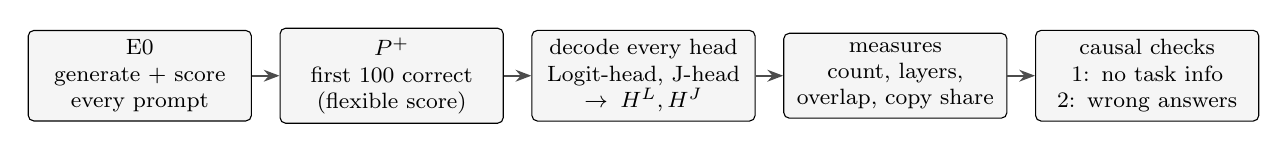
\begin{tikzpicture}[
  node distance=4mm and 3.5mm,
  box/.style={draw, rounded corners=2pt, fill=gray!8, align=center, font=\footnotesize, minimum height=9mm, text width=2.6cm},
  arr/.style={-{Stealth[length=2mm]}, thick, gray!60!black}]
\node[box] (e0) {E0\\generate + score\\every prompt};
\node[box, right=of e0] (p) {$P^{+}$\\first 100 correct\\(flexible score)};
\node[box, right=of p] (h) {decode every head\\Logit-head, J-head\\$\to H^L, H^J$};
\node[box, right=of h] (m) {measures\\count, layers,\\overlap, copy share};
\node[box, right=of m] (c) {causal checks\\1: no task info\\2: wrong answers};
\draw[arr] (e0) -- (p); \draw[arr] (p) -- (h); \draw[arr] (h) -- (m); \draw[arr] (m) -- (c);
\end{tikzpicture}
\end{center}

% ---------------------------------------------------------------------
\section{Experiments and outcomes}

\small
\begin{xltabular}{\textwidth}{@{}>{\raggedright\arraybackslash}p{2.5cm}>{\hsize=.8\hsize}L>{\hsize=1.2\hsize}Lc@{}}
\toprule
\textbf{Experiment} & \textbf{Design} & \textbf{Outcome (short)} & \\
\midrule
\endhead
\multicolumn{4}{@{}l}{\textbf{E0 --- behavioural baseline}} \\
Complex tasks & 5 tasks $\times$ 10 prompts, 300 items. & NCA, LCI answered straight away, above chance. Set Game, Op.\ Function, Tapatan always reason first. Set Game and Op.\ Function solved from rules, hardly from examples alone. Tapatan near chance everywhere. Set Game solved on 97/300 even without task info. & \mixed \\
Scoring audit & Every reply saved; strict (Fu et al.'s parser) vs flexible. & Op.\ Function 0.01--0.99 across wordings $\to$ 1.00 everywhere (missing \texttt{\textbackslash boxed}). & \yes \\
\midrule
\multicolumn{4}{@{}l}{\textbf{E2 --- complex tasks} (5 tasks $\times$ rule/example/combined $\times$ 2 readouts)} \\
Head sets & 100 prompts per style (fewer where few correct). & Heads found for every task and style, but counts not comparable with E1 (term lists 10$\times$ longer; Set Game example $P^+$ = 1 prompt). J-head again larger, layers 10--19; covers 44--91\% of Logit-head. Rule/example overlap 48--94\%. & \mixed \\
Check 1 (no task info) & Rule heads, 7 means, 11 $\alpha$, control of same answer format. & Without task info the model does not attempt the task on 4/5 tasks, and no patch changes this. Set Game: $\leq$+5 items, control as much. & \no \\
Check 2 (rules, wrong) & Rule prompts answered wrongly; control added. & Gains everywhere, but the control matches them. $\alpha=0$ alone fixes 21--23 Set Game items; on Yes/No tasks gains = pushing every answer to one label. & \no \\
\midrule
\multicolumn{4}{@{}l}{\textbf{E9 --- E8's DB set on the complex tasks} (\texttt{e9-complex-db.tex})} \\
DB set, both checks & J-head decodes the task's 30 most active words ($\geq$10\% of 700 rule prompts) and BOS attention $\leq$0.5; E2's checks, $\alpha$ 1, 2, control. & 87--109 heads, mostly shared across tasks. No task-specific effect. On Yes/No tasks a stronger one-label push than E2 (check 1: answers return, always ``Yes''; check 2: one label for all), control alike. Set Game, Tapatan: control matches or beats it. & \no \\
\bottomrule
\end{xltabular}
\normalsize

% ---------------------------------------------------------------------
\section{Hypotheses}

\begin{tabularx}{\textwidth}{@{}>{\raggedright\arraybackslash}p{3.6cm}Lc@{}}
\toprule
H1 complex $<$ simple & Causal part agrees (no task-specific effect on complex tasks); head-count part untestable (term-list length). & \mixed \\
H2 J-head $\supseteq$ Logit-head & Fails: J-head misses part of the Logit-head set on every pair. J-only heads have no task-specific effect. & \no \\
\bottomrule
\end{tabularx}

% ---------------------------------------------------------------------
\section{Design variants tried}

\small
\begin{tabularx}{\textwidth}{@{}p{1.5cm}LLL@{}}
\toprule
\textbf{Date} & \textbf{Tried first} & \textbf{Replaced by} & \textbf{Why / effect} \\
\midrule
10-27 & Rules as main style, examples secondary & Rule and example treated alike & No main condition (user decision). \\
10-27 & Drop prompts not answered straight away & Reasoning mode for Set Game, Op.\ Function, Tapatan & They are never answered straight away. \\
10-27 & Wordings/terms via ChatGPT & GPT-5.5 via Azure API, checked by hand & API instead of the chat interface. \\
10-27 & All difficulty levels & Easy level only & User decision. \\
10-27 & Reasoning mode: 10 items, $\alpha\in\{0,1,4,10\}$ & 100 items, 11 $\alpha$ values (10-30) & Same 100 items as the other tasks. \\
10-28 & Prompts and means pooled over wordings & One wording for heads, one mean per wording (Yang's code) & Matches the source exactly. \\
10-28 & Check 1 only (zero-shot) & Check 1 + check 2 (released script) & Only check 2 reproduces Yang's figures. \\
10-29 & 6,000-token replies, stop at the answer; direct vs reasoning split & 1,024 tokens for all five complex tasks, one scheme & 4/9,000 replies correct after token 1,024. \\
10-29 & Heads also read at a pre-answer position & Last prompt token only & Dropped with its results. \\
10-30 & Tapatan scored by its first line & First label anywhere & First line is the label in 1/3,000 replies. \\
10-30 & First-token (simple) / strict (complex) score for heads and checks & Flexible score; E1, E2 rerun & Strict scoring created spurious wording differences. \\
10-31 & Complex check 2 without control & Control mean added & Zero-ablation and label shifts alone gave gains. \\
\bottomrule
\end{tabularx}
\normalsize


% ---------------------------------------------------------------------
\section{What seems to work, what does not}

\begin{itemize}
\item \yes{} \textbf{Scoring matters first.} Flexible scoring removes most of the apparent wording sensitivity; always check it before reading wording effects.
\item \no{} \textbf{Complex tasks:} heads are found, but no causal check shows a task-specific effect, neither for Yang et al.'s sets (E2) nor for E8's DB rule (E9). Prompts without task info elicit no attempt (DB only brings back a ``Yes''); on wrong-answer prompts, any perturbation (zero, control, label shift) helps as much.
\item \no{} \textbf{Head counts on complex tasks} are not interpretable with long term lists and tiny $P^+$ sets.
\item \textbf{Controls are essential} on long-reasoning and Yes/No tasks: without them, check 2 looked positive.
\end{itemize}

\textbf{Not pursued:} function vectors, function-specific heads, hidden-state differences (scope, 10-27); fp32 Head-JLens fit ($\approx$136 GPU-h, declined).

\end{document}
